\chapter{Interval with triangular equality}
Before jumping in and defining what is the Pareto envelope of our set of terminals, or even saying why will we calculated it, we need to define the interval of points that respect the triangular equality.

\section{Triangular inequality/equality} %%%%%%%%%%%%%%%%%%%%%%%%%%%%%%%%%%%
\noindent The Triangula \textbf{in}equality states that:
\begin{quoting} \begin{verbatim}
  For a triangle the sum of the length of any two sides
of this triangle, must be greater than the length of the third side.
\end{verbatim} \end{quoting}
Which means that: let $abc$ be a triangle:
\begin{itemize}[noitemsep, nolistsep]
	\item{$d(a,b)+d(b,c) > d(a,c)$}
	\item{$d(a,c)+d(c,b) > d(a,b)$}
	\item{$d(b,a)+d(a,c) > d(b,c)$}
	\newline
\end{itemize}

	Now take in consideration two point \emph{a} and \emph{b}, all \emph{c} points that respect the triangular equality are the ones that do not verify the triangular inequality which means that:
\begin{itemize}[noitemsep, nolistsep]
	\item{$d(a,c)+d(c,b) \leq d(a,b)$}
	\newline
\end{itemize}

\section{Interval and metrics} %%%%%%%%%%%%%%%%%%%%%%%%%%%%%%%%%%%
	But as we defined previously d(x,y), we know that this notation depends on the metric that we use. Moreover, depending on which metric we use the set of points that will respect the triangular equality will differ. Here are some examples of this set depending on the metric used:
\begin{figure}[H]
  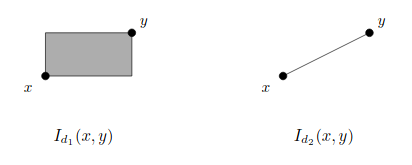
\includegraphics[width=\linewidth]{img/interval_example.png}
  \caption{Triangular equality interval depending on the metric.}
  \label{fig:interval_example}
\end{figure}

As you can see on the right, this set is just all the points on a straight line between \emph{x} and \emph{y}. In fact as we use the l2-metric (Cartesian distance) we fall back on our feet with the casual definition of the triangular inequality.

Nevertheless, on the left we see that for the l1-metric this interval is a square, with the segment [\emph{x},\emph{y}] being a diagonal of this square. And you can see that after doing the calculation we actually end up with this shape for all points that respect the triangular equality.

\section{Usage of intervals} %%%%%%%%%%%%%%%%%%%%%%%%%%%%%%%%%
Also as we will work a bit with the l1-metric, this result will be really useful for future computations.\newline

All the points that respect the triangular equality can be regrouped in a set. This set will simply be called interval between x and y for the metric $d_1$(resp. $d_{metric\_identifier}$).

It is base on this interval that we will also define the Pareto envelope of our set of terminals.

Note: As the construction of the Pareto envelope can be linked to the interval between all pair of points, and as this said interval depends on the metric that we use to calculate distances, \textbf{the Pareto envelope of a set of terminals depends on the metric that we use}.

\section{Used notation}
By defining this interval we now can have a way to start and work our way to the Pareto envelope of our set. 

This interval will be noted as: $I_{d}$.

\noindent With $d$ the identifier of the metric used to calculate this interval.